\documentclass[12pt]{article}
\usepackage{macros}
\usepackage{longtable}
\newgeometry{margin=1in}
\singlespacing
\pagestyle{fancy}
\lhead{\textsc{Stat 195 Early Forecast}}
\rhead{\textsc{Jiafeng Chen and Joon Yang}}
% \singlespacing
\begin{document}
\section*{Brief Methodology}
Let \[Y_i = \frac{\text{Republican}\% }{\text{Republican}\% + \text{Democrat}\%}\] be the proportion of Republican vote share between the major parties in district $i$, which is our outcome measure.\footnote{Assuming districts have no time dimension: i.e. Alabama-01 is represented by different $i,j$'s across two different years. We also assume for simplicity that third parties never win elections, which seems accurate in the case for 2018.} Let $x_i$ be a list of features for the district. The features we use are incumbency, gender, voting pattern in the previous presidential election, percentage of minorities, presidential approval rating and candidates' party alignment with the incumbent president, log of median income, and percent in district with Bachelor's degree or above, and one-hot encoding of states. We also include all second-order interactions of these features.

We predict (contested) elections via a two-stage process. In the first stage, we form a prior via the training data. In the second stage, we update this prior with live polling data aggregated by FiveThirtyEight. Assume the (misspecified) linear probability model
$Y_i \sim \Norm(\mu_{i0}, \sigma_0^2),$ where $\mu_{i0} = x_i^T \beta_0$. The model is misspecified since $Y_i \in [0,1]$ but Normal is supported on $\R$. Let \begin{align*}
\hat \beta_0 = \argmin_\beta \, \sum_{i=1}^{N} (y_i - x_i^T \beta)^2 + \lambda\pr{\alpha \norm{\beta}_1 + (1-\alpha) \norm{\beta}_2^2}
\end{align*}
be fitted with an elastic net regularizer over the training data, where $\lambda$ is chosen via $K$-fold cross validation and $\alpha$ is some fixed constant, say $0.9$. Let $\hat \sigma_{0i}^2 = \sum (y_j - x_j^T \hat\beta_0)^2$ be fitted as the variance of the residuals, where the sum could be over districts in the same state.\footnote{One could also estimate variance over a holdout set, which might improve bias.} Let $\hat \mu_{i0} = x_i^T \hat \beta_0$.

For a district that corresponds to an upcoming election, we form a prior 
$Y_i\sim \Norm(\hat \mu_{i0}, \hat \sigma_0^2),$ or in vector form $
Y \sim \Norm( \mu_0,  \Sigma_0)$, suppressing the hat notation. Assume a poll result is $Z \mid Y \sim \Norm(a^T Y, \sigma^2_p)$ where $a$ is $n^{-1}\bm 1$ for a nationwide poll and the $i$th standard basis for a poll conducted in the $i$th district. For each poll, we estimate $\sigma^2_p$. For the congressional generic ballot,\footnote{\url{https://projects.fivethirtyeight.com/congress-generic-ballot-polls/}} we calculate a variance implied by FiveThirtyEight's 90\% confidence interval. For a district-wide poll, we estimate $\sigma^2_p$ by using the empirical variance of polls from the same district, plus a variance implied by the Binomial model ($\frac{1}{4n}$, where $n$ is sample size in the poll). We use the latest generic ballot polling average and the latest three polls for each district. Bayesian updating yields a posterior $Y \mid Z \sim \Norm(\mu, \Sigma)$ for some $\mu, \Sigma$ that we calculate. The projected winners and probabilities in \Cref{sec:district_res} are calculated by computing the marginal probability $\P(Y_i > 0.5) = \P(\text{Republican wins $i$})$ for each $i$. The aggregate probabilities in \Cref{sec:agg_res} are calculated by drawing $10^5$ draws from $\Norm(\mu,\Sigma)$ and calculating $10^{-5}\sum_{j=1}^{10^5} \bm 1\pr{\sum_{i=1}^{n} \bm 1(Y_i^{(j)} > .5) > 217.5}$, which is the Monte Carlo probability of Republicans retaining control of the house. 

\newpage
% Note that in such a formulation, we ignore the sampling variance of $\hat \mu_{i0}$ and $\hat \sigma_0^2$,\footnote{The elastic net regularizer in the fitting method for $\beta$ makes the sampling variance of $\hat\beta_0$ difficult to compute.} instead forming a plug-in estimate, appealing to the law of large numbers.\footnote{From this point on, we drop the hat on $\mu_{i0}, \sigma_0$.} To obtain a more accurate and timely prediction for the district, we update the prior in two steps.  

% First, to take into account the ``blue wave,'' we update our prior via the generic congressional ballot.\footnote{\url{https://projects.fivethirtyeight.com/congress-generic-ballot-polls/}} Formally, we model generic congressional poll as $Z_{G} \mid Y_i \sim \Norm(Y_i, \sigma_G^2),$ where $\sigma_G^2$ is estimated from the 90\% confidence interval provided by FiveThirtyEight. We have the following data generating process: \begin{align*}
% Y &\sim \Norm(\hat \mu_0, \hat \Sigma_0)\\
% Z_G \mid Y &\sim \Norm\pr{n^{-1}1^T Y, \sigma_G^2}
% \end{align*}

% We update our prior to form an intermediate posterior: \[
% Y \mid Z_G \sim \Norm(\mu_1, \Sigma_1).
% \]
% From now on, we drop the conditioning on $Z_G$.

% Second, for some districts, we observe a number of district-specific polls $Z_{i1},\ldots,Z_{iJ_i}$.\footnote{In practice, we take the $J$ most recent polls (if available) in district $i$, where $J = 10$.} The variance across polls is much higher than implied by a simple Beta-Binomial model, where one assumes that each poll is an independent $\Bin(n_j,p)$ where $p$ is sampled from a Beta (again, approximately Normal) prior. As such, we hesitate from using a simple Beta-Binomial updating procedure and opt for the following model: We assume that poll $j$ has an independent bias $\epsilon_j \sim \Norm(0, \sigma^2_p)$, where $\sigma_p$ is estimated as the empirical variance of poll outcomes in a district: \begin{align*}
% Y &\sim \Norm(\mu_1, \Sigma_1) \quad \epsilon_j \sim \Norm(0, \sigma_p^2) \\
% Z_{ij}\mid Y_i, \epsilon_j &\sim n^{-1} \cdot \Bin(n, e_i^T Y + \epsilon_j),
% \end{align*}
% where $e_i$ is the $i$th standard basis vector. It's somewhat difficult to compute the posterior $Y \mid Z_{i1}, \ldots, Z_{iJ}$. Instead we may assume the misspecified model, justified as $n^{-1}\Bin(n, p)$ is approximately Normal when $n$ is large. \begin{align*}
% Y &\sim \Norm(\mu_{1}, \Sigma_{1}) \\
% Z_{ij} \mid Y &\sim \Norm\pr{e_i^TY, \frac{1}{4n_j} + \sigma_p^2},
% \end{align*}
% so as to (a) take advantage of Normal-Normal conjugacy and (b) ignore the dependence of $\var(Z_{ij})$ on $Y_i$. We now have the posterior by, say, sequentially Bayesian updating: \[
% Y \mid (Z_{i1},\ldots,Z_{iJ_i})_{i=1}^n \sim \Norm\pr{
%     \mu_{2}, \Sigma_{2}
% }.
% \]
% We predict $\hat Y_i = \mu_{2i}$, and, naturally \[
% \hat{\text{Winner}}_i = \begin{cases}
%     \text{Republican} & \mu_{2i} > .5 \\
%     \text{Democrat} & \mu_{2i} < .5
% \end{cases}
% \]



\appendix
\section{Projected results by district}
\label{sec:district_res}
\begin{longtable}{llr}
\toprule
          District &     Projected Winner &  Probability \\
\midrule
\endhead
\midrule
\multicolumn{3}{r}{{Continued on next page}} \\
\midrule
\endfoot

\bottomrule
\endlastfoot
        Alabama-01 &            Byrne (R) &       0.9437 \\
        Alabama-02 &             Roby (R) &       0.8779 \\
        Alabama-03 &           Rogers (R) &       0.9539 \\
        Alabama-04 &         Aderholt (R) &       0.9951 \\
        Alabama-05 &           Brooks (R) &       0.9886 \\
        Alabama-06 &           Palmer (R) &       0.9950 \\
        Alabama-07 &           Sewell (D) &       1.0000 \\
         Alaska-00 &            Young (R) &       0.9062 \\
        Arizona-01 &           Rogers (R) &       0.8118 \\
        Arizona-02 &      Kirkpatrick (D) &       0.9991 \\
        Arizona-03 &         Grijalva (D) &       0.9555 \\
        Arizona-04 &            Gosar (R) &       1.0000 \\
        Arizona-05 &            Biggs (R) &       0.9722 \\
        Arizona-06 &       Schweikert (R) &       0.9999 \\
        Arizona-07 &          Gallego (D) &       1.0000 \\
        Arizona-08 &            Lesko (R) &       0.9847 \\
        Arizona-09 &          Ferrara (R) &       0.6050 \\
       Arkansas-01 &         Crawford (R) &       1.0000 \\
       Arkansas-02 &             Hill (R) &       0.9987 \\
       Arkansas-03 &           Womack (R) &       0.9997 \\
       Arkansas-04 &        Westerman (R) &       1.0000 \\
     California-01 &          LaMalfa (R) &       0.8602 \\
     California-02 &          Huffman (D) &       0.8912 \\
     California-03 &        Garamendi (D) &       0.9122 \\
     California-04 &       McClintock (R) &       0.8579 \\
     California-05 &         Thompson (D) &       1.0000 \\
     California-06 &        Jefferson (D) &       1.0000 \\
     California-07 &             Bera (D) &       0.9661 \\
     California-08 &         Donnelly (R) &       1.0000 \\
     California-09 &         McNerney (D) &       0.9703 \\
     California-10 &           Harder (D) &       0.7081 \\
     California-11 &       DeSaulnier (D) &       0.9848 \\
     California-12 &           Pelosi (D) &       0.9998 \\
     California-13 &              Lee (D) &       1.0000 \\
     California-14 &           Speier (D) &       0.9994 \\
     California-15 &         Swalwell (D) &       0.9984 \\
     California-16 &            Costa (D) &       0.9810 \\
     California-17 &           Khanna (D) &       1.0000 \\
     California-18 &            Eshoo (D) &       0.9968 \\
     California-19 &          Lofgren (D) &       0.9981 \\
     California-20 &          Panetta (D) &       1.0000 \\
     California-21 &          Valadao (R) &       0.9448 \\
     California-22 &            Nunes (R) &       0.9999 \\
     California-23 &         McCarthy (R) &       0.7099 \\
     California-24 &         Carbajal (D) &       0.7035 \\
     California-25 &             Hill (D) &       0.5623 \\
     California-26 &         Brownley (D) &       0.7666 \\
     California-27 &             Witt (D) &       1.0000 \\
     California-28 &           Schiff (D) &       0.9864 \\
     California-29 &         Cárdenas (D) &       0.9678 \\
     California-30 &          Sherman (D) &       0.9690 \\
     California-31 &          Aguilar (D) &       0.9519 \\
     California-32 &       Napolitano (D) &       0.9976 \\
     California-33 &             Lieu (D) &       0.9905 \\
     California-34 &            Gomez (D) &       1.0000 \\
     California-35 &           Torres (D) &       0.9903 \\
     California-36 &             Ruiz (D) &       0.9080 \\
     California-37 &             Bass (D) &       0.9998 \\
     California-38 &          Sánchez (D) &       0.9966 \\
     California-39 &         Cisneros (D) &       0.9278 \\
     California-40 &    Roybal-Allard (D) &       1.0000 \\
     California-41 &           Takano (D) &       0.9912 \\
     California-42 &          Calvert (R) &       0.6121 \\
     California-43 &           Waters (D) &       0.9998 \\
     California-44 &            Brown (D) &       1.0000 \\
     California-45 &           Porter (D) &       0.7104 \\
     California-46 &           Correa (D) &       0.9382 \\
     California-47 &        Lowenthal (D) &       0.9918 \\
     California-48 &      Rohrabacher (R) &       0.7144 \\
     California-49 &            Levin (D) &       0.9975 \\
     California-50 &           Hunter (R) &       0.8935 \\
     California-51 &           Vargas (D) &       0.8783 \\
     California-52 &           Peters (D) &       0.9884 \\
     California-53 &            Davis (D) &       0.9735 \\
       Colorado-01 &          DeGette (D) &       0.9953 \\
       Colorado-02 &               Yu (R) &       0.6428 \\
       Colorado-03 &           Tipton (R) &       0.9047 \\
       Colorado-04 &             Buck (R) &       0.9558 \\
       Colorado-05 &          Lamborn (R) &       0.7863 \\
       Colorado-06 &             Crow (D) &       0.8873 \\
       Colorado-07 &       Perlmutter (D) &       0.7680 \\
    Connecticut-01 &           Larson (D) &       0.9923 \\
    Connecticut-02 &         Courtney (D) &       0.7857 \\
    Connecticut-03 &          DeLauro (D) &       0.9816 \\
    Connecticut-04 &            Himes (D) &       0.9832 \\
    Connecticut-05 &            Hayes (D) &       0.5873 \\
       Delaware-00 &        Rochester (D) &       1.0000 \\
        Florida-01 &            Gaetz (R) &       0.7632 \\
        Florida-02 &             Dunn (R) &       0.8150 \\
        Florida-03 &             Yoho (R) &       0.7214 \\
        Florida-04 &       Rutherford (R) &       0.8029 \\
        Florida-05 &           Lawson (D) &       0.9961 \\
        Florida-06 &            Waltz (R) &       0.8650 \\
        Florida-07 &           Murphy (D) &       0.7432 \\
        Florida-08 &            Posey (R) &       0.8233 \\
        Florida-09 &             Soto (D) &       0.9047 \\
        Florida-10 &          Demings (D) &       1.0000 \\
        Florida-11 &          Webster (R) &       0.8721 \\
        Florida-12 &        Bilirakis (R) &       0.9993 \\
        Florida-13 &            Crist (D) &       0.7810 \\
        Florida-14 &           Castor (D) &       1.0000 \\
        Florida-15 &            Spano (R) &       0.5816 \\
        Florida-16 &         Buchanan (R) &       0.9992 \\
        Florida-17 &           Steube (R) &       0.8274 \\
        Florida-18 &             Mast (R) &       0.9808 \\
        Florida-19 &           Rooney (R) &       0.9295 \\
        Florida-20 &         Hastings (D) &       1.0000 \\
        Florida-21 &          Frankel (D) &       1.0000 \\
        Florida-22 &           Deutch (D) &       0.8801 \\
        Florida-23 &          Schultz (D) &       0.8910 \\
        Florida-24 &           Wilson (D) &       1.0000 \\
        Florida-25 &      Diaz-Balart (R) &       0.9963 \\
        Florida-26 &  Mucarsel-Powell (D) &       0.5451 \\
        Florida-27 &          Shalala (D) &       0.5672 \\
        Georgia-01 &           Carter (R) &       0.9836 \\
        Georgia-02 &           Bishop (D) &       0.9970 \\
        Georgia-03 &         Ferguson (R) &       0.9956 \\
        Georgia-04 &          Johnson (D) &       1.0000 \\
        Georgia-05 &            Lewis (D) &       1.0000 \\
        Georgia-06 &           Handel (R) &       0.9226 \\
        Georgia-07 &          Woodall (R) &       0.9576 \\
        Georgia-08 &            Scott (R) &       1.0000 \\
        Georgia-09 &          Collins (R) &       0.9999 \\
        Georgia-10 &             Hice (R) &       0.9952 \\
        Georgia-11 &       Loudermilk (R) &       0.9917 \\
        Georgia-12 &            Allen (R) &       0.9798 \\
        Georgia-13 &            Scott (D) &       1.0000 \\
        Georgia-14 &           Graves (R) &       1.0000 \\
         Hawaii-01 &             Case (D) &       0.9952 \\
         Hawaii-02 &          Gabbard (D) &       0.9671 \\
          Idaho-01 &          Fulcher (R) &       0.9972 \\
          Idaho-02 &          Simpson (R) &       1.0000 \\
       Illinois-01 &             Rush (D) &       0.9999 \\
       Illinois-02 &            Kelly (D) &       1.0000 \\
       Illinois-03 &         Lipinski (D) &       0.8759 \\
       Illinois-04 &           Garcia (D) &       0.8801 \\
       Illinois-05 &          Quigley (D) &       0.9481 \\
       Illinois-06 &           Roskam (R) &       0.5243 \\
       Illinois-07 &            Davis (D) &       1.0000 \\
       Illinois-08 &   Krishnamoorthi (D) &       0.9771 \\
       Illinois-09 &       Schakowsky (D) &       0.9919 \\
       Illinois-10 &        Schneider (D) &       0.9787 \\
       Illinois-11 &           Foster (D) &       0.9774 \\
       Illinois-12 &             Bost (R) &       0.9981 \\
       Illinois-13 &            Davis (R) &       0.9524 \\
       Illinois-14 &         Hultgren (R) &       0.9403 \\
       Illinois-15 &          Shimkus (R) &       0.9339 \\
       Illinois-16 &        Kinzinger (R) &       0.9271 \\
       Illinois-17 &           Bustos (D) &       0.7207 \\
       Illinois-18 &           LaHood (R) &       0.8914 \\
        Indiana-01 &        Visclosky (D) &       0.9007 \\
        Indiana-02 &         Walorski (R) &       0.9559 \\
        Indiana-03 &            Banks (R) &       0.9993 \\
        Indiana-04 &            Baird (R) &       0.9242 \\
        Indiana-05 &           Brooks (R) &       0.8775 \\
        Indiana-06 &            Pence (R) &       0.9605 \\
        Indiana-07 &           Carson (D) &       0.9945 \\
        Indiana-08 &          Bucshon (R) &       0.9762 \\
        Indiana-09 &    Hollingsworth (R) &       0.9716 \\
           Iowa-01 &       Finkenauer (D) &       0.7665 \\
           Iowa-02 &         Loebsack (D) &       0.9823 \\
           Iowa-03 &            Young (R) &       0.5987 \\
           Iowa-04 &             King (R) &       0.9941 \\
         Kansas-01 &         Marshall (R) &       0.9923 \\
         Kansas-02 &            Davis (D) &       0.8405 \\
         Kansas-03 &           Davids (D) &       0.8445 \\
         Kansas-04 &            Estes (R) &       0.9612 \\
       Kentucky-01 &            Comer (R) &       0.9762 \\
       Kentucky-02 &          Guthrie (R) &       0.9818 \\
       Kentucky-03 &          Yarmuth (D) &       0.9148 \\
       Kentucky-04 &           Massie (R) &       0.9878 \\
       Kentucky-05 &           Rogers (R) &       0.9834 \\
       Kentucky-06 &             Barr (R) &       0.7338 \\
      Louisiana-01 &          Scalise (R) &       0.9822 \\
      Louisiana-02 &         Richmond (D) &       1.0000 \\
      Louisiana-03 &         Guillory (R) &       0.9627 \\
      Louisiana-04 &          Johnson (R) &       0.9026 \\
      Louisiana-05 &          Abraham (R) &       0.9138 \\
      Louisiana-06 &           Graves (R) &       0.9657 \\
          Maine-01 &          Pingree (D) &       1.0000 \\
          Maine-02 &           Golden (D) &       0.5062 \\
       Maryland-01 &           Harris (R) &       0.9021 \\
       Maryland-02 &    Ruppersberger (D) &       0.9980 \\
       Maryland-03 &         Sarbanes (D) &       0.9984 \\
       Maryland-04 &            Brown (D) &       1.0000 \\
       Maryland-05 &            Hoyer (D) &       0.9995 \\
       Maryland-06 &            Trone (D) &       0.6709 \\
       Maryland-07 &         Cummings (D) &       1.0000 \\
       Maryland-08 &           Raskin (D) &       0.9975 \\
  Massachusetts-01 &             Neal (D) &       1.0000 \\
  Massachusetts-02 &         McGovern (D) &       0.9878 \\
  Massachusetts-03 &           Trahan (D) &       0.6887 \\
  Massachusetts-04 &          Kennedy (D) &       1.0000 \\
  Massachusetts-05 &            Clark (D) &       1.0000 \\
  Massachusetts-06 &          Moulton (D) &       0.9881 \\
  Massachusetts-07 &         Pressley (D) &       1.0000 \\
  Massachusetts-08 &            Lynch (D) &       1.0000 \\
  Massachusetts-09 &          Keating (D) &       0.9384 \\
       Michigan-01 &          Bergman (R) &       0.9366 \\
       Michigan-02 &         Huizenga (R) &       0.9753 \\
       Michigan-03 &            Amash (R) &       0.8428 \\
       Michigan-04 &        Moolenaar (R) &       0.9580 \\
       Michigan-05 &           Kildee (D) &       0.8468 \\
       Michigan-06 &            Upton (R) &       0.9759 \\
       Michigan-07 &          Walberg (R) &       0.9096 \\
       Michigan-08 &           Bishop (R) &       0.8928 \\
       Michigan-09 &          Stearns (R) &       0.5957 \\
       Michigan-10 &         Mitchell (R) &       0.9594 \\
       Michigan-11 &          Stevens (D) &       0.8978 \\
       Michigan-12 &          Dingell (D) &       0.9276 \\
       Michigan-13 &            Tlaib (D) &       1.0000 \\
       Michigan-14 &         Lawrence (D) &       1.0000 \\
      Minnesota-01 &         Hagedorn (R) &       0.9888 \\
      Minnesota-02 &            Craig (D) &       0.8612 \\
      Minnesota-03 &         Phillips (D) &       0.9959 \\
      Minnesota-04 &         McCollum (D) &       0.9997 \\
      Minnesota-05 &             Omar (D) &       0.9316 \\
      Minnesota-06 &            Emmer (R) &       0.9613 \\
      Minnesota-07 &         Peterson (D) &       0.9900 \\
      Minnesota-08 &          Stauber (R) &       0.9899 \\
    Mississippi-01 &            Kelly (R) &       1.0000 \\
    Mississippi-02 &         Thompson (D) &       1.0000 \\
    Mississippi-03 &            Guest (R) &       1.0000 \\
    Mississippi-04 &          Palazzo (R) &       1.0000 \\
       Missouri-01 &             Clay (D) &       1.0000 \\
       Missouri-02 &           Wagner (R) &       0.9827 \\
       Missouri-03 &      Luetkemeyer (R) &       0.9996 \\
       Missouri-04 &         Hartzler (R) &       0.9971 \\
       Missouri-05 &          Cleaver (D) &       0.9940 \\
       Missouri-06 &           Graves (R) &       0.9988 \\
       Missouri-07 &             Long (R) &       0.9980 \\
       Missouri-08 &            Smith (R) &       0.9990 \\
        Montana-00 &        Gianforte (R) &       0.9904 \\
       Nebraska-01 &      Fortenberry (R) &       0.9729 \\
       Nebraska-02 &            Bacon (R) &       0.9968 \\
       Nebraska-03 &            Smith (R) &       0.9532 \\
         Nevada-01 &            Titus (D) &       1.0000 \\
         Nevada-02 &           Amodei (R) &       0.9817 \\
         Nevada-03 &              Lee (D) &       0.5961 \\
         Nevada-04 &         Horsford (D) &       0.7008 \\
  New Hampshire-01 &           Pappas (D) &       0.5641 \\
  New Hampshire-02 &           Kuster (D) &       0.9999 \\
     New Jersey-01 &         Norcross (D) &       0.9853 \\
     New Jersey-02 &         Van Drew (D) &       0.9930 \\
     New Jersey-03 &        MacArthur (R) &       0.5258 \\
     New Jersey-04 &            Smith (R) &       0.8790 \\
     New Jersey-05 &       Gottheimer (D) &       0.7508 \\
     New Jersey-06 &          Pallone (D) &       0.9981 \\
     New Jersey-07 &       Malinowski (D) &       0.9337 \\
     New Jersey-08 &            Sires (D) &       0.9997 \\
     New Jersey-09 &         Pascrell (D) &       0.9985 \\
     New Jersey-10 &            Payne (D) &       1.0000 \\
     New Jersey-11 &         Sherrill (D) &       0.9987 \\
     New Jersey-12 &          Coleman (D) &       0.9998 \\
     New Mexico-01 &          Haaland (D) &       0.9559 \\
     New Mexico-02 &          Herrell (R) &       0.6293 \\
     New Mexico-03 &            Lujan (D) &       1.0000 \\
       New York-01 &           Zeldin (R) &       0.9944 \\
       New York-02 &             King (R) &       0.7832 \\
       New York-03 &           Suozzi (D) &       0.9774 \\
       New York-04 &             Rice (D) &       0.9904 \\
       New York-05 &            Meeks (D) &       1.0000 \\
       New York-06 &             Meng (D) &       1.0000 \\
       New York-07 &        Velázquez (D) &       1.0000 \\
       New York-08 &         Jeffries (D) &       1.0000 \\
       New York-09 &           Clarke (D) &       1.0000 \\
       New York-10 &           Nadler (D) &       0.9987 \\
       New York-11 &          Donovan (R) &       0.8481 \\
       New York-12 &          Maloney (D) &       0.9996 \\
       New York-13 &        Espaillat (D) &       1.0000 \\
       New York-14 &    Ocasio-Cortez (D) &       0.9914 \\
       New York-15 &          Serrano (D) &       1.0000 \\
       New York-16 &            Engel (D) &       1.0000 \\
       New York-17 &            Lowey (D) &       1.0000 \\
       New York-18 &          Maloney (D) &       0.9161 \\
       New York-19 &          Delgado (D) &       0.5809 \\
       New York-20 &            Tonko (D) &       0.9301 \\
       New York-21 &         Stefanik (R) &       0.9296 \\
       New York-22 &           Tenney (R) &       0.5790 \\
       New York-23 &             Reed (R) &       0.8954 \\
       New York-24 &            Katko (R) &       0.8353 \\
       New York-25 &          Morelle (D) &       1.0000 \\
       New York-26 &          Higgins (D) &       0.9727 \\
       New York-27 &          Collins (R) &       0.9086 \\
 North Carolina-01 &      Butterfield (D) &       0.9998 \\
 North Carolina-02 &          Coleman (D) &       0.5117 \\
 North Carolina-03 &            Jones (R) &       1.0000 \\
 North Carolina-04 &            Price (D) &       0.9990 \\
 North Carolina-05 &             Foxx (R) &       0.9229 \\
 North Carolina-06 &           Walker (R) &       0.8581 \\
 North Carolina-07 &           Rouzer (R) &       0.6217 \\
 North Carolina-08 &           Hudson (R) &       0.7578 \\
 North Carolina-09 &           Harris (R) &       0.5323 \\
 North Carolina-10 &          McHenry (R) &       0.9526 \\
 North Carolina-11 &          Meadows (R) &       0.9840 \\
 North Carolina-12 &            Adams (D) &       0.9999 \\
 North Carolina-13 &             Budd (R) &       0.9432 \\
   North Dakota-00 &        Armstrong (R) &       1.0000 \\
           Ohio-01 &           Chabot (R) &       0.9741 \\
           Ohio-02 &         Wenstrup (R) &       0.8480 \\
           Ohio-03 &           Beatty (D) &       0.9989 \\
           Ohio-04 &           Jordan (R) &       0.9298 \\
           Ohio-05 &            Latta (R) &       0.9539 \\
           Ohio-06 &          Johnson (R) &       0.9476 \\
           Ohio-07 &            Gibbs (R) &       0.9643 \\
           Ohio-08 &         Davidson (R) &       0.9113 \\
           Ohio-09 &           Kaptur (D) &       0.9571 \\
           Ohio-10 &           Turner (R) &       0.6972 \\
           Ohio-11 &            Fudge (D) &       1.0000 \\
           Ohio-12 &        Balderson (R) &       0.7839 \\
           Ohio-13 &             Ryan (D) &       0.8111 \\
           Ohio-14 &            Joyce (R) &       0.8866 \\
           Ohio-15 &          Stivers (R) &       0.9366 \\
           Ohio-16 &         Gonzalez (R) &       0.8639 \\
       Oklahoma-01 &             Hern (R) &       0.9994 \\
       Oklahoma-02 &           Mullin (R) &       0.9983 \\
       Oklahoma-03 &            Lucas (R) &       1.0000 \\
       Oklahoma-04 &             Cole (R) &       1.0000 \\
       Oklahoma-05 &          Russell (R) &       1.0000 \\
         Oregon-01 &         Bonamici (D) &       0.9841 \\
         Oregon-02 &           Walden (R) &       0.9899 \\
         Oregon-03 &       Blumenauer (D) &       1.0000 \\
         Oregon-04 &          DeFazio (D) &       0.8985 \\
         Oregon-05 &         Callahan (R) &       0.9391 \\
   Pennsylvania-01 &          Wallace (D) &       0.9390 \\
   Pennsylvania-02 &            Boyle (D) &       1.0000 \\
   Pennsylvania-03 &            Evans (D) &       0.5970 \\
   Pennsylvania-04 &            David (R) &       0.8486 \\
   Pennsylvania-05 &              Kim (R) &       0.7688 \\
   Pennsylvania-06 &         McCauley (R) &       0.7684 \\
   Pennsylvania-07 &             Wild (D) &       0.9974 \\
   Pennsylvania-08 &       Cartwright (D) &       1.0000 \\
   Pennsylvania-09 &           Meuser (R) &       0.9659 \\
   Pennsylvania-10 &            Perry (R) &       0.9285 \\
   Pennsylvania-11 &          Smucker (R) &       0.9823 \\
   Pennsylvania-12 &           Marino (R) &       0.9676 \\
   Pennsylvania-13 &          Ottaway (D) &       0.9795 \\
   Pennsylvania-14 &           Boerio (D) &       0.8416 \\
   Pennsylvania-15 &         Thompson (R) &       0.8850 \\
   Pennsylvania-16 &            Kelly (R) &       0.9972 \\
   Pennsylvania-17 &             Lamb (D) &       1.0000 \\
   Pennsylvania-18 &            Doyle (D) &       1.0000 \\
   Rhode Island-01 &        Cicilline (D) &       0.9972 \\
   Rhode Island-02 &         Langevin (D) &       0.9614 \\
 South Carolina-01 &        Arrington (R) &       0.9419 \\
 South Carolina-02 &           Wilson (R) &       0.9530 \\
 South Carolina-03 &           Duncan (R) &       0.9873 \\
 South Carolina-04 &          Timmons (R) &       0.9064 \\
 South Carolina-05 &           Norman (R) &       0.9553 \\
 South Carolina-06 &          Clyburn (D) &       0.9999 \\
 South Carolina-07 &             Rice (R) &       0.9685 \\
   South Dakota-00 &          Johnson (R) &       0.9993 \\
      Tennessee-01 &              Roe (R) &       0.9978 \\
      Tennessee-02 &         Burchett (R) &       0.9830 \\
      Tennessee-03 &      Fleischmann (R) &       0.9927 \\
      Tennessee-04 &       DesJarlais (R) &       0.9952 \\
      Tennessee-05 &           Cooper (D) &       0.8470 \\
      Tennessee-06 &             Rose (R) &       0.9936 \\
      Tennessee-07 &            Green (R) &       0.9760 \\
      Tennessee-08 &          Kustoff (R) &       0.9762 \\
      Tennessee-09 &            Cohen (D) &       1.0000 \\
          Texas-01 &          Gohmert (R) &       0.9061 \\
          Texas-02 &           Litton (D) &       0.5955 \\
          Texas-03 &            Burch (D) &       0.5861 \\
          Texas-04 &        Ratcliffe (R) &       0.9473 \\
          Texas-05 &           Gooden (R) &       0.6724 \\
          Texas-06 &           Wright (R) &       0.8620 \\
          Texas-07 &        Culberson (R) &       0.5983 \\
          Texas-08 &            Brady (R) &       0.9495 \\
          Texas-09 &            Green (D) &       1.0000 \\
          Texas-10 &           McCaul (R) &       0.8241 \\
          Texas-11 &          Conaway (R) &       0.9665 \\
          Texas-12 &          Granger (R) &       1.0000 \\
          Texas-13 &       Thornberry (R) &       0.9585 \\
          Texas-14 &            Weber (R) &       0.8992 \\
          Texas-15 &         Gonzalez (D) &       0.8031 \\
          Texas-16 &        Seeberger (R) &       0.7069 \\
          Texas-17 &           Flores (R) &       0.9932 \\
          Texas-18 &              Lee (D) &       0.9998 \\
          Texas-19 &        Arrington (R) &       0.8770 \\
          Texas-20 &           Castro (D) &       1.0000 \\
          Texas-21 &              Roy (R) &       0.9996 \\
          Texas-22 &            Olson (R) &       0.7188 \\
          Texas-23 &             Hurd (R) &       0.9985 \\
          Texas-24 &         Marchant (R) &       0.7023 \\
          Texas-25 &         Williams (R) &       0.9393 \\
          Texas-26 &          Burgess (R) &       0.9186 \\
          Texas-27 &            Cloud (R) &       0.9602 \\
          Texas-28 &          Cuellar (D) &       1.0000 \\
          Texas-29 &          Aronoff (R) &       0.7069 \\
          Texas-30 &          Johnson (D) &       1.0000 \\
          Texas-31 &           Carter (R) &       0.9999 \\
          Texas-32 &           Allred (D) &       0.8241 \\
          Texas-33 &           Veasey (D) &       0.8431 \\
          Texas-34 &             Vela (D) &       0.6385 \\
          Texas-35 &          Doggett (D) &       0.8276 \\
          Texas-36 &            Babin (R) &       0.9617 \\
           Utah-01 &           Bishop (R) &       1.0000 \\
           Utah-02 &          Stewart (R) &       1.0000 \\
           Utah-03 &           Curtis (R) &       1.0000 \\
           Utah-04 &             Love (R) &       0.9128 \\
        Vermont-00 &            Welch (D) &       1.0000 \\
       Virginia-01 &          Wittman (R) &       0.8668 \\
       Virginia-02 &           Taylor (R) &       0.6855 \\
       Virginia-03 &            Scott (D) &       1.0000 \\
       Virginia-04 &         McEachin (D) &       0.9957 \\
       Virginia-05 &         Cockburn (D) &       0.6231 \\
       Virginia-06 &            Cline (R) &       0.8657 \\
       Virginia-07 &             Brat (R) &       0.5299 \\
       Virginia-08 &            Beyer (D) &       0.9991 \\
       Virginia-09 &         Griffith (R) &       0.9746 \\
       Virginia-10 &           Wexton (D) &       0.8683 \\
       Virginia-11 &         Connolly (D) &       0.9993 \\
     Washington-01 &          DelBene (D) &       0.9885 \\
     Washington-02 &           Larsen (D) &       1.0000 \\
     Washington-03 &          Beutler (R) &       0.9578 \\
     Washington-04 &         Newhouse (R) &       0.7732 \\
     Washington-05 &          Rodgers (R) &       0.9380 \\
     Washington-06 &           Kilmer (D) &       0.9506 \\
     Washington-07 &          Jayapal (D) &       1.0000 \\
     Washington-08 &            Rossi (R) &       0.7611 \\
     Washington-09 &            Smith (D) &       1.0000 \\
     Washington-10 &             Heck (D) &       0.9834 \\
  West Virginia-01 &         McKinley (R) &       1.0000 \\
  West Virginia-02 &           Mooney (R) &       1.0000 \\
  West Virginia-03 &           Miller (R) &       0.8775 \\
      Wisconsin-01 &            Steil (R) &       0.8612 \\
      Wisconsin-02 &            Pocan (D) &       1.0000 \\
      Wisconsin-03 &             Kind (D) &       0.8023 \\
      Wisconsin-04 &            Moore (D) &       1.0000 \\
      Wisconsin-05 &    Sensenbrenner (R) &       0.8126 \\
      Wisconsin-06 &         Grothman (R) &       0.9069 \\
      Wisconsin-07 &            Duffy (R) &       0.8676 \\
      Wisconsin-08 &        Gallagher (R) &       0.8487 \\
        Wyoming-00 &           Cheney (R) &       0.9660 \\
\end{longtable}


\section{Projected total seats}
\label{sec:agg_res}

The probability of Republicans retaining the majority is \textbf{0.273} and the probability of Democrats retaining the majority is \textbf{0.727}, which are slightly more in favor of Republicans than reported by FiveThirtyEight and is less in favor of Republicans than the latest betting odds on PredictIt.\footnote{\url{https://www.predictit.org/markets/detail/2704/Which-party-will-control-the-House-after-2018-midterms}}
% \begin{figure}[tb]
%     \centering
%     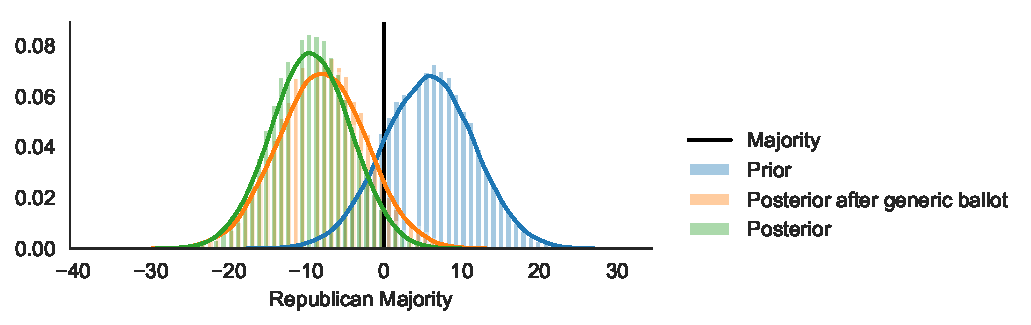
\includegraphics{rep_seats.pdf}
%     \caption{Projected Republican seat holdings}
%     \label{fig:seats}
% \end{figure}
% \section{Fitting Method}

% \section{Results}

% \section{Uncertainty and robustness}

% \section{Conclusion}
\end{document}
